
\documentclass[10pt]{beamer}
\usetheme{Warsaw}
\usecolortheme{orchid}
\usepackage{mycros}
\mode<presentation>
{
	\usetheme{Warsaw}
	\setbeamercovered{transparent}
}

\title{Spectral rigidity of some arithmetic surfaces}
\author{Justin Katz}
\institute{Purdue University}
\newcommand{\Stuff}{\ensuremath{\mathbf{Stuff}}}
\newcommand{\stuff}{\ensuremath{\text{stuff}}}
\newcommand{\Things}{\ensuremath{\mathbf{Things}}}
\newcommand{\thing}{\ensuremath{\text{thing}}}
\newcommand{\Lspec}{{\rm Lspec}}
\newcommand{\Tspec}{{\rm Tspec}}

\begin{document}
\frame{\titlepage}
\begin{frame} \frametitle{Abstract nonsense}
	\begin{itemize}[<+->]
					\item Generally speaking, stuff is hard to understand.
					\item A framework: \pause  introduce an invariant
						\[ F : \Stuff \to \Things \] \pause
					\item For a $\thing \in \Things$\pause, study the fiber 
					\[ F^{-1} (\thing) \subset \Stuff\] \pause
					\item Rigidity:  \pause $F^\inv(\thing)$ is a singleton  \onslide+<11->(bonus points: when $F$ is not-so-complicated and $\Things$ not so mysterious.)
	\end{itemize}
	\end{frame}
\begin{frame}  \frametitle{Concrete nonsense}
In this talk: \pause 
	   \begin{itemize}
					\item<2-> $ \Stuff:= \text{closed Riemannian manifolds } (M,g) $
					\item<3-> $\Things:=\text{discretely supported measures on } \R_{\geq 0}$
					\item<4-> \onslide+<4->{ $F(\cdot) := \spec_{(\cdot)}$, where
		 				\[ \spec_{M,g} ( \{\lambda\} ) = \dim \ker_{L^2(M,\dop \vol_g))} (\Delta_{M,g} - \lambda 
		 				)\] }  \onslide+<5-> {$F(\cdot) := \Lspec_{(\cdot)}$, where
		 				\[ \spec_{M,g} ( \{\ell \} ) =  \# \{ \gamma \subset \pi_1(M): \ell_g(\gamma)= \ell  \}  \]} 
	\end{itemize} \onslide+<7->
\begin{thm}
	Certain hyperbolic $2$ manifolds are absolutely spectrally rigid. Principal congruence covers of surfaces arising from maximal orders  in quaternion algebras with type number 1 are spectrally rigid. 
\end{thm}
	\end{frame}
\begin{frame} \frametitle{Background}
A (very hard) question: \pause Which measures $\mu$ arise as $\spec_{M,g}$ for some $(M,g)$?  \pause \\ 
 Examples:
			\begin{itemize}[<+->]
				\item For a flat torus $\Rbb^n / L$.
					\[ \spec_{\Rbb^n/L, \dop x^2}  = \sum_{x \in L^*}  \delta_{-||x||^2 }   \]
				where $L^*$ is the lattice dual to $L$. \pause  Case  $L=\Zbb^n$: which integers are sums of $n$ squares? \pause In how many ways?  \pause
				\item For a round $n-1$ dimensional sphere $S^{n-1}$: \pause 
					\[ \spec_{S^{n-1} }  =   \sum_{a \geq 0} \frac{(a+n/2 -1) \prod_{j=1}^{n-3} (a+j)}{(n/2-1)\cdot (n-3)! }\delta_{a^2 + (n-2) a }\]
			\end{itemize}
\pause
Generally speaking, one shouldn't expect a closed form expression for spectra. 
\end{frame}%%%%%%%%%%%%%%%%%%%%%%%%%%%%%%%%%%%%%%%%%%%%%%%%%%%%%%%%%%%%%%%%%%%%%%%%%%
\begin{frame} \frametitle{Isospectrality}
			\begin{itemize}[<+->]
				\item  Two Riemannian manifolds $(M_1,g_1)$ and  $(M_2,g_2)$ are said to be \textbf{isospectral}, or belong to the same \textbf{spectral genus}, when $\spec_{M_1,g_1} = \spec_{M_2,g_2}$.
				\item $(M,g)$ is \textbf{spectrally rigid} if its spectral genus is a singleton. 
				\item Mark Kac asked in  1966 whether all Riemannian manifolds are spectrally rigid. 
				\item Milnor, two years prior:\onslide+<5> no! 
			\end{itemize}
\end{frame}
\begin{frame} %milnor
	\begin{figure}
	\centering
	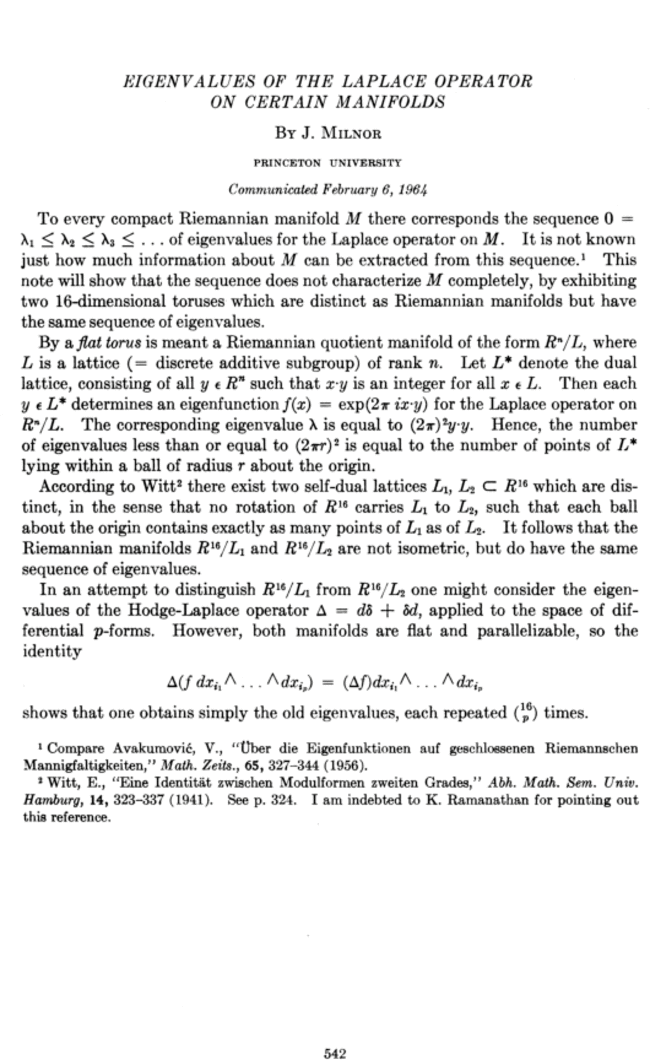
\includegraphics[scale=.3]{milnor}
\end{figure}
\end{frame}%%%%%%%%%%%%%%%%%%%%%%%%%%%%%%%%%%%%%%%%%%%%%%%%%%%%%%%%%%%%%%%%%%%%%%%%%%
\begin{frame} \frametitle{Heat invariants}
	\begin{itemize}[<+->]
		\item A \textbf{spectral invariant}, or \textbf{audible property}, is one which is constant along 
		spectral 
		genera.
		\item A key source of spectral invariants: \pause the trace of the \textbf{heat kernel} 
			\[ \Theta_{M,g} (t) =  \int e^{-\lambda t } \dop \spec_{M,g}(\lambda) \]  
		\begin{thm}[Minakshisundaram-Pleijel] 
			\begin{itemize}[<+->]
				\item There are constants $a_k(M,g)=a_k$ such that, as $t \to 0^+$ one has 
					\[ \Theta_{M,g} (t) = (4 \pi t)^{-\dim(M)/2} \sum_{k =1}^\infty a_k t^k .\]
				\item The coefficients $a_k$ are integrals of polynomials in curvatures and its derivatives. 
				The first 
				three are: 
					\[ a_0 = \vol(M),\,\pause a_1 = \frac{1}{6} \int_M \tau,\pause \, a_2 = \frac{1}{360} \int_M 
					5\tau^2 
					- 2 |{\rm Ric} | ^2 - 10 |R|^2. \]
			\end{itemize}
			\end{thm}
	\end{itemize}
	\end{frame}%%%%%%%%%%%%%%%%%%%%%%%%%%%%%%%%%%%%%%%%%%%%%%%%%%%%%%%%%%%%%%%%%%%%%%%%%%
\begin{frame} \frametitle{Heat invariants: consequences}
	\begin{itemize}[<+->]
		\item Evidently, dimension, volume, and total (scalar) curvature are spectral invariants. 
		\item Consequently anything isospectral to a  \alt<6->{\textbf{hyperbolic} surface}{surface} 
		is a 
		\alt<6->{\textbf{hyperbolic} surface}{surface}\onslide+<4->{, \textbf{to which it is 
		homeomorphic}!}
		\item In fact: by Gauss-Bonnet $a_1$ for a surface is a topological invariant. 
		\item Comparing $a_1$ and $a_2$, any variation in curvature is audible.   
	\end{itemize}	
\end{frame}%%%%%%%%%%%%%%%%%%%%%%%%%%%%%%%%%%%%%%%%%%%%%%%%%%%%%%%%%%%%%%%%%%%%%%%%%%
\begin{frame} \frametitle{Hyperbolic surfaces: Fuchsian uniformization}
	\begin{itemize}[<+->]
				\item  A compact hyperbolic surface admits a description as $\Gamma \lmod \Hbb$ for a 
				cocompact lattice $\Gamma \in \PSL(2,\Rbb) \approx \Isom^+ (\Hbb)$, where $\Hbb$ is the 
				hyperbolic plane. 
				\item $\Hbb \to \Gamma \lmod \Hbb $ is the universal covering map, $\Gamma$ is the deck 
				group,  and identifies with the fundamental group of the quotient.
				\item Elements of $\Gamma$ are \emph{pointed homotopy} classes of closed curves, 
				\pause 
				conjugacy classes in $\Gamma$ are  \emph{free homotopy} classes of closed curves on 
				the 
				compact surface. \pause
				\item Within each such free homotopy class is a unique geodesic representative.  \pause 
				Its length 
				$\ell$ is related to the trace $t$ of a representative matrix by $2e^{\ell/2} = t + \sqrt{t^2 
				-4}$. 
				\item Define the \textbf{length} and \textbf{trace} spectrum of $\Gamma \lmod \Hbb$: 
					\[ \Lspec =  \sum_{\ell \in \ell(\Gamma)}  m(\ell)\delta_\ell, \quad \Tspec = \sum _{t \in 
					\Tr(\Gamma)} m(t) 
					\delta_t  \] 
				\pause where $m(\ell)$ and $m(t)$ are the number of geodesics  on $\Gamma \lmod \Hbb$ 
				of 
				length $\ell$ or trace $t$ respectively. 
				
	\end{itemize}
\end{frame}%%%%%%%%%%%%%%%%%%%%%%%%%%%%%%%%%%%%%%%%%%%%%%%%%%%%%%%%%%%%%%%%%%%%%%%%%%
\begin{frame} \frametitle{Hyperbolic surfaces: Arithmeticity}
 \begin{itemize}[<+->]
 	\item A hyperbolic surface $\Gamma \lmod \Hbb$ is \textbf{arithmetic} if there exists 
 	\begin{itemize}[<+->]
 		\item A totally real number field $k$,
 		\item a quaternion algebra $A$ over $k$ such that there is a unique real place $\rho: k \to \Rbb$ such that $A \otimes_\rho \Rbb = M(2,\Rbb)$, and
 		\item a maximal order $\Ocal \leq A$ with norm $1$ units $\Ocal^1$
 	\end{itemize}
 \pause such that $\Gamma$ is commensurable to the image of $\rho(\Ocal^1) $ in $ 
 \PSL(2,\Rbb)$. 
 \pause
 \item Classic example: 
			\[ k = \Qbb,\,  A = M(2,\Qbb),\, \Ocal = M(2,\Zbb), \, \Gamma = \PSL(2,\Zbb)  \]
 \item Key fact: the isomorphism class of the quternion algebra $A$ is a complete invariant of the commensurability class of an arithmetic surface. 
 \end{itemize}
\end{frame}%%%%%%%%%%%%%%%%%%%%%%%%%%%%%%%%%%%%%%%%%%%%%%%%%%%%%%%%%%%%%%%%%%%%%%%%%%
\begin{frame} \frametitle{Hyperbolic surfaces: audibility of arithmeticity}
Selberg Trace formula:  for a closed hyperbolic surface, knowledge of eigenvalue spectrum is equivalent to knowledge of the length spectrum, \pause equivalent to knowledge of trace spectrum. \pause  
\begin{thm}[Takeuchi]
	A closed hyperbolic surface $\Gamma \lmod \Hbb$ is arithmetic and derived from a quaternion algebra if and only if  
	\begin{itemize} [<+->]
		\item $k=\Qbb(\Tr(\Gamma))$  is a number field, 
		\item $\Tr(\Gamma)$ is contained in its integers, and 
		\item for any nonidentity embedding $\phi: k \to \Cbb$, the image $\phi(\Tr(\Gamma))$ is bounded.   
	\end{itemize}
\end{thm}
\pause
Anything isospectral to a compact hyperbolic \textbf{arithmetic} surface is a compact 
hyperbolic \textbf{arithmetic} surface \onslide+<8->{\textbf{to which it is 
commensurable}}\onslide+<9->,{ (by a 
theorem due to Reid).} 
\end{frame}%%%%%%%%%%%%%%%%%%%%%%%%%%%%%%%%%%%%%%%%%%%%%%%%%%%%%%%%%%%%%%%%%%%%%%%%%%



\begin{frame}%%%%%%%%%%%%%%%%%%%%%%%%%%%%%%%%%%%%%%%%%%%%%%%%%%%%%%%%%%%%%%%%%%%%%%%%%
	\centering
	 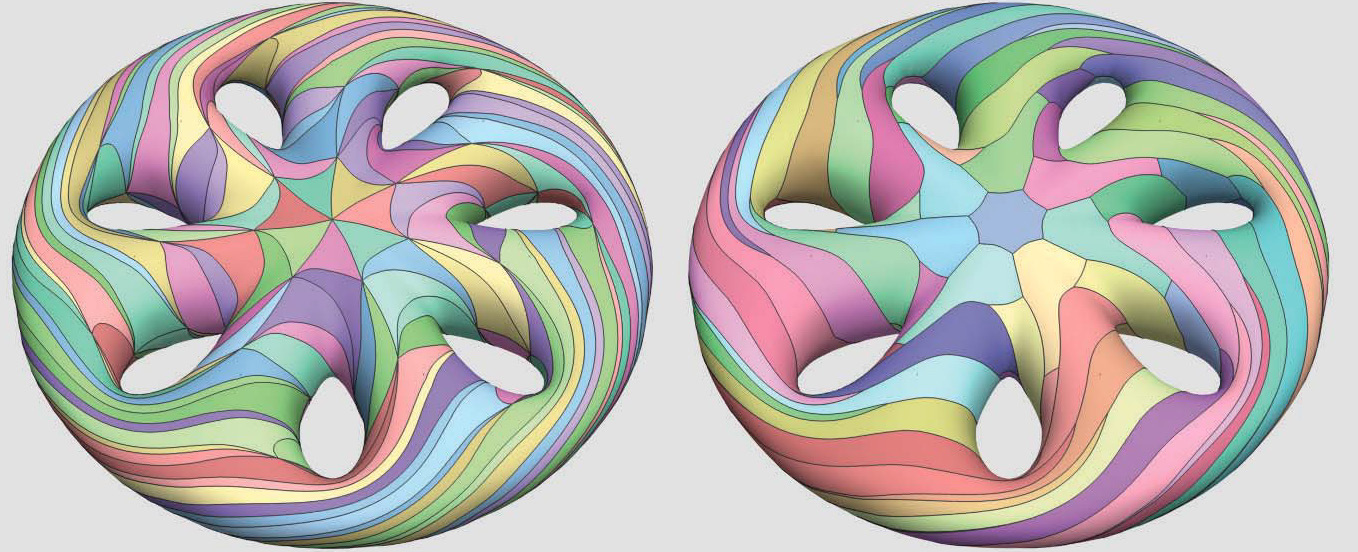
\includegraphics[scale=.5]{vanWijkGenus7.jpg}
\end{frame}%%%%%%%%%%%%%%%%%%%%%%%%%%%%%%%%%%%%%%%%%%%%%%%%%%%%%%%%%%%%%%%%%%%%%%%%%%
\end{document}


